\subsection{Использование компонентов и пресетов}
\label{sec:manual:components_manual}

Как говорилось ранее, основным инструментом приложения и единственным инструментом для отображения визуальной части создаваемых макетов является грид.

Использование этого алгоритма на практике крайне незатруднительно, что значительно понижает <<порог вхождения>> пользователей.

\subsubsection{Компоненты}
\

Применение компонентов осуществляется по алгоритму <<Drag-n-drop>>, что в переводе с английского означает буквально <<Тащи и бросай>>. Наглядно этот процесс показан на рисунке~\ref{sec:manual:manual_using_pallet}.

\begin{figure}[ht]
	\centering
    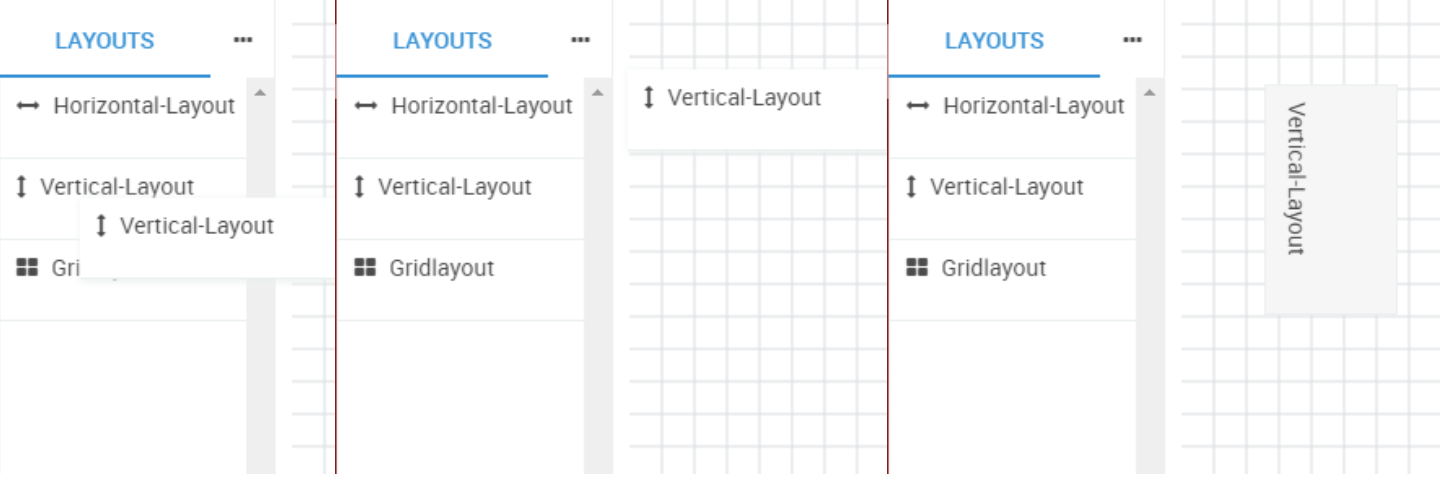
\includegraphics[scale=0.43]{manual_using_pallet.png}
    \caption{Перетягивание компонента на грид}
    \label{sec:manual:manual_using_pallet}
\end{figure}

Непосредственно на грид могут быть перетянуты лишь компоненты типа <<layout>> или пользовательские шаблоны. При попытке перетянуть другие компоненты на грид в правом верхнем углу экрана будет появляться сообщение об ошибке, как показано на рисунке~\ref{sec:manual:manual_dnd_error_message}.

\begin{figure}[ht]
	\centering
    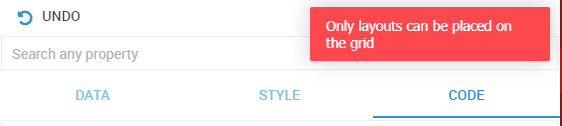
\includegraphics[scale=0.6]{manual_dnd_error_message.png}
    \caption{Сообщение об ошибке при перетягивании компонента на грид}
    \label{sec:manual:manual_dnd_error_message}
\end{figure}

При перетягивании компонента, не относящегося к типу <<layout>>, на другой компонент, относящийся к типу <<layout>>, последний будет подсвечен (если не будет иметь дочерние элементы в момент перетягивания), как показано на рисунке~\ref{sec:manual:manual_dnd_to_layout}.

\begin{figure}[ht]
	\centering
    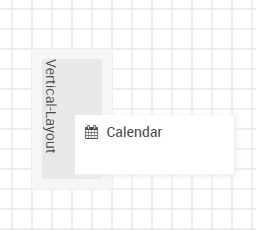
\includegraphics[scale=0.6]{manual_dnd_to_layout.png}
    \caption{Сообщение об ошибке при перетягивании компонента на грид}
    \label{sec:manual:manual_dnd_to_layout}
\end{figure}

Результатом процесса перетягивания будет помещение перетягиваемого компонента внутрь объекта, на который он был перетянут. Данный результат продемонстрирован на рисунке~\ref{sec:manual:manual_dnd_to_layout}.

\begin{figure}[ht]
  \centering
    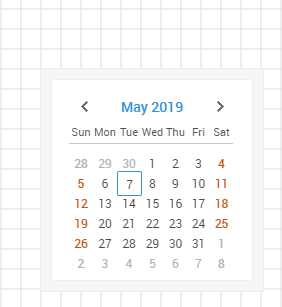
\includegraphics[scale=0.6]{manual_dnd_result.png}
    \caption{Результат перетягивания компонента на лэйаут}
    \label{sec:manual:manual_dnd_result}
\end{figure}

Стоит отметить, что данное программное средство не ставит никакие ограничения по вложенности компонентов. То есть, никто и ничто не помешает пользователю помесить лайэаут в лэйаут, который находится в другом лэйауте и т.д. Пример представлен на рисунке~\ref{sec:manual:manual_components_dnd}.

Таким образом, можно сделать вывод, что данная функциональность была реализована должным образом и ни в коей мере не будет <<сковывать>> пользователя в подобного рода действиях.

\begin{figure}[ht]
  \centering
    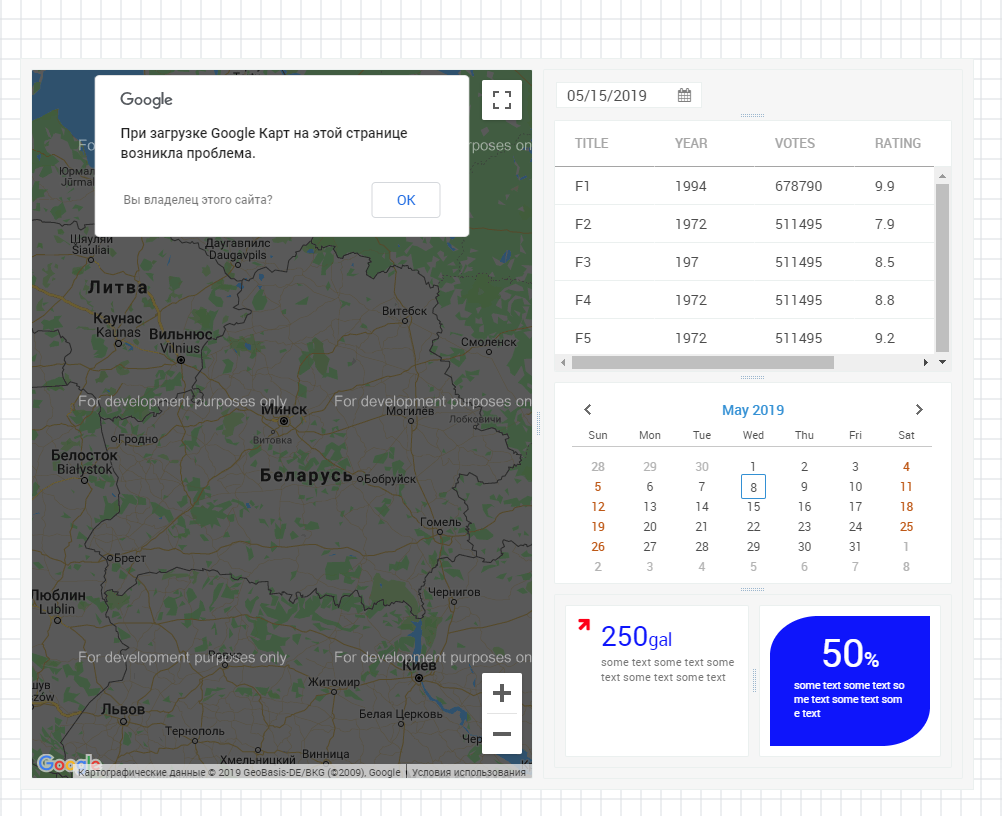
\includegraphics[scale=0.5]{manual_components_dnd.png}
    \caption{Комплексный компонент, состоящий из двух лэйаутов и их содержимого}
    \label{sec:manual:manual_components_dnd}
\end{figure}

\subsubsection{Пресеты}
\

Как уже говорилось, для использования пресетов существует одноименная вкладка в component pallet. После ее открытия появляется список доступных пресетов, однако если их нет, отобразится соответствующее сообщение, как показано на рисунке~\ref{sec:manual:manual_no_presets_found}.

\begin{figure}[ht]
\centering
    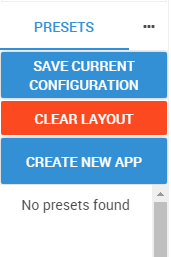
\includegraphics[scale=0.8]{manual_no_presets_found.png}
    \caption{Результат перетягивания компонента на лэйаут}
    \label{sec:manual:manual_no_presets_found}
\end{figure}

\pagebreak
Для сохранения текущего макета в пресет необходимо нажать на кнопку <<SAVE CURRENT CONFIGURATION>>, выбрав затем имя для пресета. На данный момент присутствует простейшая валидация на ввод пустой строки, как продемонстрировано на рисунке~\ref{sec:manual:manual_preset_add_err}.

\begin{figure}[ht]
  \centering
    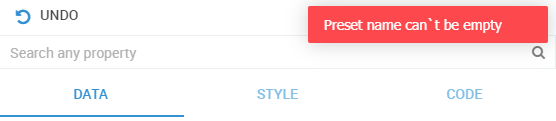
\includegraphics[scale=0.8]{manual_preset_add_err.png}
    \caption{Результат перетягивания компонента на лэйаут}
    \label{sec:manual:manual_preset_add_err}
\end{figure}

В случае, если уже существует пресет с введенным именем, также будет выведено соответствующее сообщение об ошибке, как продемонстрировано на рисунке~\ref{sec:manual:manual_preset_add_err_already_exists}.

\begin{figure}[ht]
  \centering
    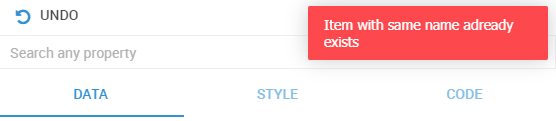
\includegraphics[scale=0.8]{manual_preset_add_err_already_exists.png}
    \caption{Результат перетягивания компонента на лэйаут}
    \label{sec:manual:manual_preset_add_err_already_exists}
\end{figure}

Если же введенное имя проходит валидацию, то пресет сохраняется в списке, который сраху же перерисовывается, добавляя новый элемент в самом низу. Содержимое грида при этом не очищается, поэтому пользователь сможет продолжить создание макета.

Результатом применения пресета будет содержимое грида на момент сохранения пресета и соответствующее сообщение в правом верхнем углу экрана, как показано на рисунке~\ref{sec:manual:manual_preset_creating}.

\begin{figure}[ht]
  \centering
    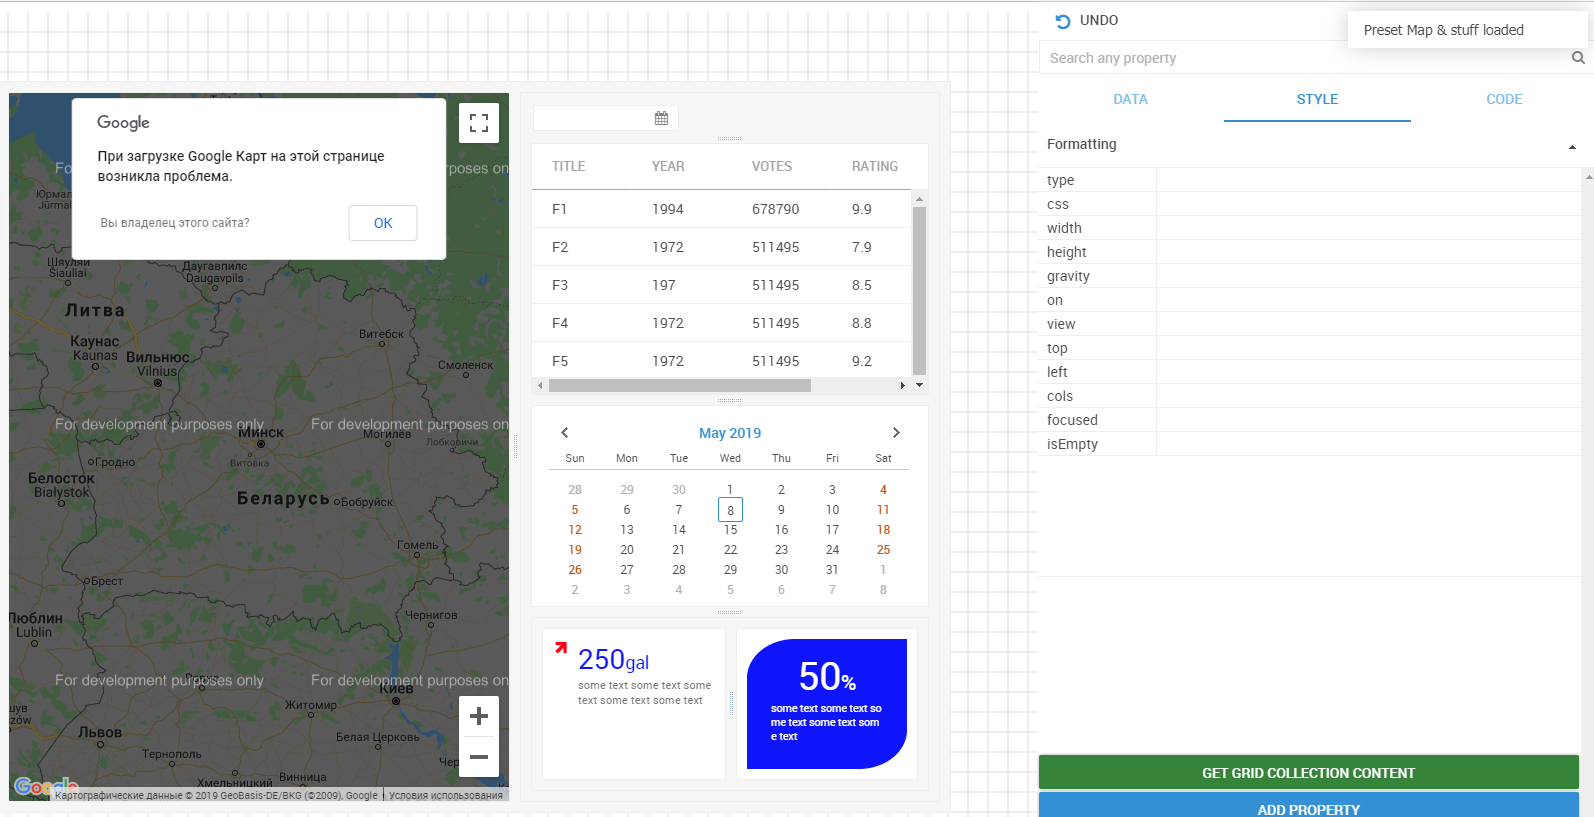
\includegraphics[scale=0.35]{manual_preset_creating.png}
    \caption{Результат применения пресета}
    \label{sec:manual:manual_preset_creating}
\end{figure}
